\documentclass[11pt,a4paper]{article}

% ========== packages ==========
\usepackage[utf8]{inputenc}
\usepackage[T1]{fontenc}
\usepackage{lmodern}
\usepackage[margin=1in]{geometry}
\usepackage{amsmath,amssymb,amsfonts}
\usepackage{mathtools}
\usepackage{booktabs}
\usepackage{multirow}
\usepackage{graphicx}
\usepackage{xcolor}
\usepackage{tikz}
\usetikzlibrary{positioning,fit,calc}
\usepackage{pgfplots}
\pgfplotsset{compat=1.17}
\usepackage{algorithm}
\usepackage{algpseudocode}
\usepackage{hyperref}
\hypersetup{colorlinks=true,linkcolor=blue!60!black,citecolor=green!50!black,urlcolor=blue!70!black}
\usepackage{cleveref}
\usepackage{enumitem}
\usepackage{caption}
\usepackage{subfig}
\usepackage{float}

% ========== custom commands ==========
\newcommand{\T}{\mathsf{T}}
\newcommand{\F}{\mathsf{F}}
\newcommand{\pME}{\operatorname{pME}}
\newcommand{\SL}{\mathcal{L}_{\text{SDD}}}
\newcommand{\LTNloss}{\mathcal{L}_{\text{LTN}}}
\newcommand{\Lfact}{\mathcal{L}_{\text{fact}}}

\title{%
  Logic Tensor Networks for Logically Consistent\\
  Large Language Models}
\author{
  Anishwar Chakraborty \\
  Travis Tran \\
  \textit{CS 273P -- Machine Learning and Data Mining} \\
  University of California, Irvine
}
\date{March 2026}

\begin{document}
\maketitle

% ======================================================================
% ABSTRACT
% ======================================================================
\begin{abstract}
Large language models (LLMs) can assign plausible truth values to
natural-language statements, but they often contradict themselves when
reasoning across related facts.  We explore whether Logic Tensor Networks
(LTNs) can reduce these inconsistencies while keeping factual accuracy
intact.  Our approach treats a pretrained LLM as a soft truth-value estimator
and feeds its output probabilities into differentiable logical constraints
covering universal quantification, conjunction, disjunction, equivalence,
and exclusive-or.

The training objective combines a supervised factual loss with a logic-based
constraint-satisfaction loss.  We compare four configurations:
(i)~a \emph{base} LLM with no logic training,
(ii)~an \emph{SDD} model that uses Sentential Decision Diagrams for
propositional semantic loss,
(iii)~an \emph{LTN} model driven by fuzzy first-order logic constraints,
and (iv)~a \emph{hybrid} model that combines both SDD and LTN losses.
On BeliefBank with LLaMA~3.2-1B, SDD achieves the best factuality
(F1\,=\,0.88) and consistency (0.87).  The hybrid model reaches the highest
fuzzy rule satisfaction (0.70).  LTN-only fails to converge
(F1\,=\,0.14), mainly because of sensitivity to the logic-weight
hyperparameter.  The untrained baseline scores near random (F1\,=\,0.18).
These results show the promise of neuro-symbolic training for LLM belief
coherence, but also reveal how hard it is to balance fuzzy-logic losses
with factual supervision.
\end{abstract}

% ======================================================================
% 1  INTRODUCTION
% ======================================================================
\section{Introduction}

\subsection{Problem Definition and Motivation}

Large language models pick up broad factual knowledge during pretraining,
but they are prone to logical self-contradiction across related
facts~\cite{kassner2021beliefbank}.  An LLM might correctly state that
``a dog is a mammal'' and ``a mammal is warm-blooded,'' yet deny that
``a dog is warm-blooded.''  Each answer is plausible on its own; taken
together, they violate a simple transitivity rule.

Current fixes sit at two extremes.  Full-scale fine-tuning is expensive
and risks catastrophic forgetting.  Offloading reasoning to an external
symbolic solver is brittle and breaks end-to-end differentiability.  We
propose a middle ground using Logic Tensor Networks (LTNs).  LTNs
are a neuro-symbolic framework that turns first-order logic formulas into
differentiable tensor computations.  They rely on fuzzy logic, a
generalisation of classical Boolean logic where truth values range
continuously over $[0,1]$ instead of being strictly true or false.  By
using LTN constraint satisfaction as a training signal, we can steer the
LLM toward logically coherent beliefs without needing a separate reasoning
engine at inference time.

\medskip
\noindent\textbf{Research question.}
Can LTN-style constraint satisfaction improve logical consistency without
hurting factual accuracy?  And does it generalise better than the existing
SDD-based approach once we introduce richer rules (XOR, conjunction,
disjunction, equivalence)?

\subsection{Related Work}

\paragraph{Logically Consistent LMs (LoCo-LM).}
Calanzone et al.~\cite{calanzone2025loco} introduce a neuro-symbolic loss
that enforces implication and negation constraints on BeliefBank using
Sentential Decision Diagrams (SDDs).  An SDD is a compact data
structure that represents a Boolean function as a directed acyclic graph.
It supports conjunction, disjunction, negation, and model counting in
time polynomial in the diagram size.  Their loss enumerates every
satisfying assignment of a propositional formula compiled into an SDD and
penalises the LLM for placing probability mass on unsatisfying worlds.
SDDs are principled, but they are strictly propositional. They
cannot express quantified rules, and diagram size can blow up
exponentially for constraints like XOR or multi-antecedent conjunctions.

\paragraph{Logic Tensor Networks.}
LTN~\cite{badreddine2022ltn} is a framework for differentiable
first-order logic.  It represents logical formulas through fuzzy semantics
over real-valued tensors.  Quantified rules are aggregated with the
pMeanError operator, a differentiable generalisation of the
universal quantifier that focuses gradient pressure on the
least-satisfied groundings.  The LTNtorch library~\cite{ltntorch2024}
provides a stable ``product configuration'' using the product t-norm for
conjunction (truth values are multiplied), probabilistic sum for
disjunction, and Reichenbach implication.  This combination is
well-suited to gradient-based optimisation.

\paragraph{BeliefBank.}
Kassner et al.~\cite{kassner2021beliefbank} build a structured knowledge
base of 12{,}363 true/false statements about 85 animal and plant entities.
It comes with a constraint graph of 4{,}058 implication and negation edges
derived from ConceptNet.  We use BeliefBank as our evaluation dataset and
extend its constraint graph with richer rule types.

\paragraph{Semantic Loss.}
Xu et al.~\cite{xu2018semantic} derive a differentiable loss that bridges
neural-network outputs with propositional constraints.  It sums over the
satisfying models of a formula compiled into an SDD.  Both LoCo-LM and our
own SDD and hybrid configurations rely on this loss.

% ======================================================================
% 2  METHODOLOGY
% ======================================================================
\section{Methodology}

\subsection{Dataset Description}

\paragraph{BeliefBank (original).}
The original dataset has 12{,}363 true/false statements about 85 entities
(animals and plants).  A constraint graph links these statements with
4{,}058 directed edges, each encoding an implication or negation
(e.g.\ \texttt{IsA,mammal} $\Rightarrow$
\texttt{HasProperty,warm\-blooded}).  We feed this graph directly into the
SDD-based experiments.

\paragraph{BeliefBank Augmented.}
We extend the constraint set with approximately 600--700 new rules of five
types not expressible as simple binary implications:
\begin{itemize}[nosep]
  \item \textbf{XOR}: exactly one of a set of predicates should hold
        (e.g.\ an entity is either domestic or wild, but not both);
  \item \textbf{AND-implies}: a conjunction of antecedents implies a
        consequent;
  \item \textbf{OR-implies}: a disjunction of antecedents implies a
        consequent;
  \item \textbf{Equivalence}: two predicates are logically equivalent;
  \item \textbf{Universal}: a single-antecedent implication.
\end{itemize}
We generate these rules by prompting an LLM with the full truth table of
each entity's predicates and then validate them against the silver-fact
labels.  After deduplication, the combined rule set (legacy + augmented) is
used for both LTN and hybrid training and for evaluation across all
configurations.

\paragraph{Data splits.}
Train/validation/test splits are done by entity (not randomly by
fact) so that generalisation is tested on unseen entities.  In practice,
antecedent predicates form the training set and consequent-only predicates
form the test set, with 10\% of the antecedent facts held out for
validation.

\subsection{Model Design}

\subsubsection{Base LLM as a Soft Truth Estimator}

We use LLaMA~3.2-1B~\cite{llama32} as the backbone.  To fit the model in
GPU memory we load it in 4-bit NF4 quantisation via BitsAndBytes, which
stores each weight in only 4~bits and cuts memory use by roughly
$4\times$.  On top of the frozen quantised weights we apply Low-Rank
Adaptation (LoRA,~$r{=}8$, $\alpha{=}2$, dropout\,=\,0.05).  LoRA
injects small trainable low-rank matrices into every linear layer, so
only a tiny fraction of parameters are updated during fine-tuning.

Given a natural-language statement~$s$, we build a prompt of the form

\begin{center}
\texttt{You can answer only with "yes" or "no". Is the fact true?\\
Fact: \{s\} Answer:}
\end{center}

\noindent We then extract the softmax probability of the target token
(``yes'' or ``true'', depending on prompt format) at the last position:
\begin{equation}\label{eq:prob}
  P_\theta(s) \;=\; \operatorname{softmax}\!\bigl(
    \mathbf{h}_L^{(\text{last})}\,W_{\text{vocab}}
  \bigr)[\texttt{target\_token}],
\end{equation}
Here $\mathbf{h}_L^{(\text{last})}$ is the hidden state at the final
position of the $L$-layer transformer and $W_{\text{vocab}}$ is the
unembedding matrix.  Because the whole pipeline is differentiable with
respect to the LoRA parameters, $P_\theta(s)$ can serve as the grounding
for all downstream logical operators.

% ========== architecture diagram ==========
\begin{figure}[H]
\centering
\resizebox{\textwidth}{!}{%
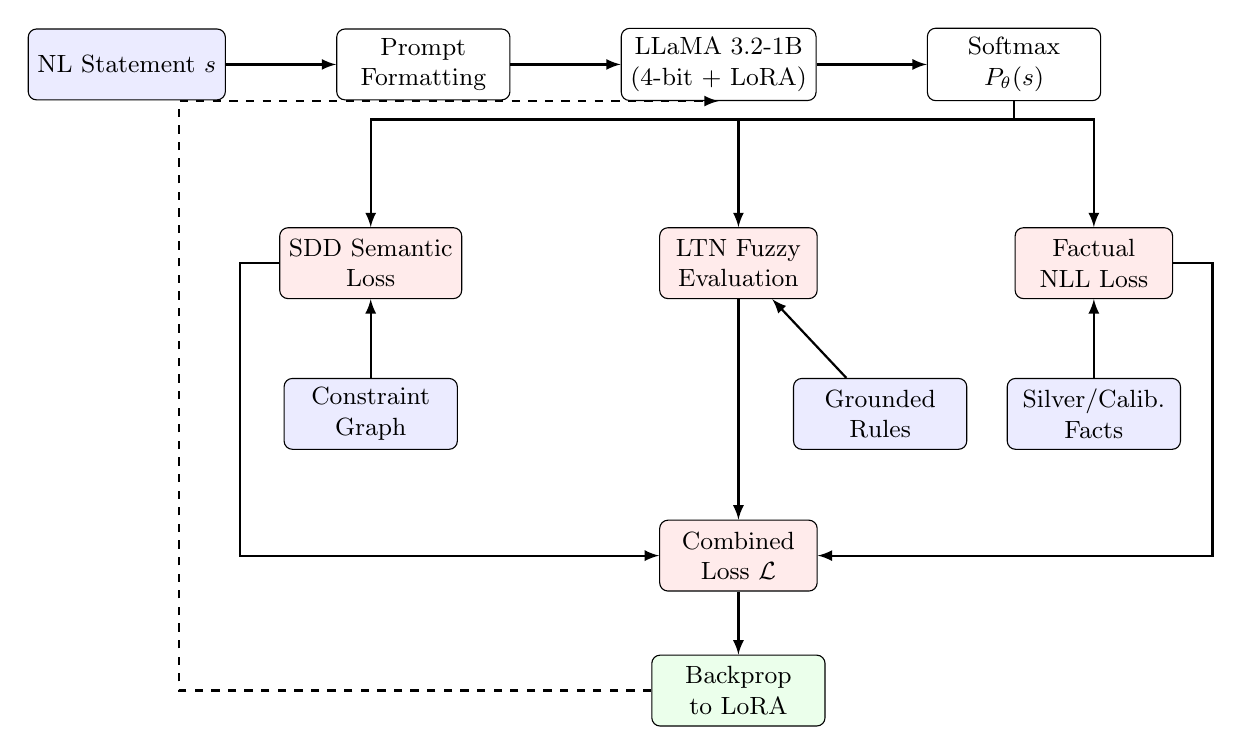
\begin{tikzpicture}[
    node distance=1.2cm,
    box/.style={draw, rounded corners=3pt, minimum height=0.9cm,
                minimum width=2.2cm, align=center, font=\small},
    loss/.style={draw, rounded corners=3pt, minimum height=0.9cm,
                 minimum width=2.0cm, align=center, font=\small,
                 fill=red!8},
    data/.style={draw, rounded corners=3pt, minimum height=0.9cm,
                 minimum width=2.2cm, align=center, font=\small,
                 fill=blue!8},
    arr/.style={-latex, thick},
  ]
  % Row 1: input
  \node[data] (stmt) {NL Statement $s$};
  \node[box, right=1.4cm of stmt] (prompt) {Prompt\\Formatting};
  \node[box, right=1.4cm of prompt] (llm) {LLaMA 3.2-1B\\(4-bit + LoRA)};
  \node[box, right=1.4cm of llm] (softmax) {Softmax\\$P_\theta(s)$};

  % Row 2: losses (wide spacing so data nodes below don't collide)
  \node[loss, below=1.6cm of softmax, xshift=-3.5cm] (ltn) {LTN Fuzzy\\Evaluation};
  \node[loss, left=2.5cm of ltn] (sdd) {SDD Semantic\\Loss};
  \node[loss, right=2.5cm of ltn] (fact) {Factual\\NLL Loss};

  % Data inputs (below each loss; rules offset right, room thanks to wider spacing)
  \node[data, below=1.0cm of sdd] (constr) {Constraint\\Graph};
  \node[data, below=1.0cm of ltn, xshift=1.8cm] (rules) {Grounded\\Rules};
  \node[data, below=1.0cm of fact] (facts) {Silver/Calib.\\Facts};

  % Row 3: combined loss (below the data row)
  \node[loss, below=2.8cm of ltn] (comb) {Combined\\Loss $\mathcal{L}$};

  % Arrows: main pipeline
  \draw[arr] (stmt) -- (prompt);
  \draw[arr] (prompt) -- (llm);
  \draw[arr] (llm) -- (softmax);

  % Arrows: softmax to losses
  \draw[arr] (softmax) -- ++(0,-0.7) -| (sdd.north);
  \draw[arr] (softmax) -- ++(0,-0.7) -| (ltn.north);
  \draw[arr] (softmax) -- ++(0,-0.7) -| (fact.north);

  % Arrows: data to losses (straight up)
  \draw[arr] (constr) -- (sdd);
  \draw[arr] (rules) -- (ltn);
  \draw[arr] (facts) -- (fact);

  % Arrows: losses to combined (routed around data nodes)
  \draw[arr] (sdd.west) -- ++(-0.5,0) |- (comb.west);
  \draw[arr] (ltn) -- (comb);
  \draw[arr] (fact.east) -- ++(0.5,0) |- (comb.east);

  % Backprop arrow
  \node[box, below=0.8cm of comb, fill=green!8] (bp) {Backprop\\to LoRA};
  \draw[arr] (comb) -- (bp);
  \draw[arr, dashed] (bp.west) -- ++(-6.0,0) |- (llm.south);

\end{tikzpicture}%
}
\caption{System architecture.  A statement is formatted into a prompt and
  passed through the quantised LLaMA model.  The output probability
  $P_\theta(s)$ feeds into three loss components, whose combined gradient
  updates only the LoRA adapters.}
\label{fig:arch}
\end{figure}

\subsubsection{SDD Semantic Loss}

Following Xu et al.~\cite{xu2018semantic} and Calanzone et
al.~\cite{calanzone2025loco}, we compile each constraint into an SDD and
enumerate its satisfying models.  For a formula $\varphi$ over Boolean
variables $x_1, \dots, x_n$ the semantic loss is
\begin{equation}\label{eq:sdd}
  \SL \;=\; -\log\!\Biggl(
    \sum_{w \,\models\, \varphi}
    \prod_{i=1}^{n} p_i^{\,w_i}\,(1-p_i)^{1-w_i}
    + \epsilon
  \Biggr),
\end{equation}
where $p_i = P_\theta(s_i)$ is the LLM's probability for statement~$s_i$,
$w_i \in \{0,1\}$ is the truth assignment in world~$w$, and
$\epsilon = 10^{-10}$ prevents numerical underflow.

Our SDD constraint manager supports four modes, combined in the
\texttt{all} configuration used in experiments:
\begin{align}
  \text{Implication:}  \quad & \neg x_1 \lor x_2, \label{eq:impl}\\
  \text{Inverse impl.:}\quad & x_2 \lor \neg x_1, \label{eq:inv}\\
  \text{Negation:}     \quad & (x_i \oplus \overline{x}_i)
                               \;\text{for both } i \in \{1,2\}, \label{eq:neg}\\
  \text{All:}          \quad & \eqref{eq:impl} \land \eqref{eq:inv}
                               \land \eqref{eq:neg}. \label{eq:all}
\end{align}
When ground-truth labels are available for either side of a constraint, we
condition the SDD on those assignments.  This restricts the set of
satisfying worlds and gives a stronger training signal.

\subsubsection{LTN Fuzzy Logic Evaluation}

We use the stable product configuration from
LTNtorch~\cite{ltntorch2024}.  Every truth value is clamped to
$[\epsilon, 1{-}\epsilon]$ before each operation so that gradients do not
vanish.

\paragraph{Fuzzy connectives.}
\begin{align}
  \lnot_f(x) &= 1 - x, \label{eq:fnot}\\[4pt]
  \land_f(x_1, \dots, x_k) &= \prod_{i=1}^{k}
    \operatorname{clamp}(x_i), \label{eq:fand}\\[4pt]
  \lor_f(x_1, \dots, x_k) &= 1 - \prod_{i=1}^{k}
    \bigl(1 - \operatorname{clamp}(x_i)\bigr), \label{eq:for}\\[4pt]
  (A \Rightarrow_f C) &= A \cdot C + (1 - A) \cdot \gamma,
    \qquad \gamma = 0.5, \label{eq:fimpl}\\[4pt]
  (L \Leftrightarrow_f R) &= 1 - |L - R|, \label{eq:fequiv}
\end{align}
where $\operatorname{clamp}(x) = \min(\max(x, \epsilon), 1{-}\epsilon)$.
The implication floor $\gamma{=}0.5$ replaces the vacuous-truth behaviour
of standard Reichenbach implication ($1{-}A{+}AC$).  Without it, rules
whose antecedent is near zero would be trivially satisfied and produce no
useful gradient.  The floor keeps the truth value non-trivial and
maintains gradient pressure during training.

\paragraph{Rule evaluation.}
Each rule type maps to a specific combination of connectives:
\begin{center}
\begin{tabular}{@{}ll@{}}
\toprule
\textbf{Rule type} & \textbf{Fuzzy semantics} \\
\midrule
\texttt{universal} / \texttt{and\_implies}
  & $\land_f(\text{ants}) \Rightarrow_f \land_f(\text{cons})$ \\
\texttt{or\_implies}
  & $\lor_f(\text{ants}) \Rightarrow_f \land_f(\text{cons})$ \\
\texttt{equivalence}
  & $\land_f(\text{ants}) \Leftrightarrow_f \land_f(\text{cons})$ \\
\texttt{xor}
  & $1 - \operatorname{ReLU}\!\bigl(\sum_i x_i - 1\bigr)$ \\
\bottomrule
\end{tabular}
\end{center}

\paragraph{pMeanError aggregation.}
Given rule truth values $u_1, \dots, u_n$, the \emph{pMeanError}
aggregator~\cite{badreddine2022ltn} computes
\begin{equation}\label{eq:pme}
  \pME_p(u_1, \dots, u_n)
  \;=\; 1 - \left(
    \frac{1}{n}\sum_{i=1}^{n}(1 - u_i)^p
  \right)^{\!1/p}\!,
\end{equation}
with $p{=}2$ (the default for balanced gradient distribution).  Increasing
$p$ shifts focus toward the hardest-to-satisfy rules; $p{\to}\infty$
recovers the minimum.

\paragraph{LTN logic loss.}
\begin{equation}\label{eq:ltnloss}
  \LTNloss \;=\; -\log\!\bigl(\pME_p(u_1, \dots, u_n)\bigr).
\end{equation}

\subsubsection{Factual Supervision Loss}

For a set of ground-truth facts $\{(s_j, y_j)\}$ where $y_j \in \{0,1\}$,
the factual loss is the negative log-likelihood of the target token:
\begin{equation}\label{eq:factloss}
  \Lfact \;=\; -\frac{1}{|B|}\sum_{j \in B}
    \log P_\theta\!\bigl(
      \text{token}_{y_j} \mid \text{prompt}(s_j)
    \bigr),
\end{equation}
where $\text{token}_{y_j}$ is ``yes'' when $y_j{=}1$ and ``no'' when
$y_j{=}0$.

\subsubsection{Combined Training Objectives}

We train three configurations with different composite losses:

\paragraph{SDD-only.}
\begin{equation}\label{eq:loss-sdd}
  \mathcal{L}_{\text{SDD-only}}
  = \lambda_{\text{sdd}}\,\SL.
\end{equation}
Because the SDD loss already conditions on ground-truth labels when they
are available, it implicitly encodes factual grounding.  No separate
factual term is needed.

\paragraph{LTN-only.}
\begin{equation}\label{eq:loss-ltn}
  \mathcal{L}_{\text{LTN-only}}
  = \lambda_{\text{ltn}}\,\LTNloss
  + \lambda_{\text{fact}}\,\Lfact.
\end{equation}

\paragraph{Hybrid.}
\begin{equation}\label{eq:loss-hybrid}
  \mathcal{L}_{\text{Hybrid}}
  = \lambda_{\text{sdd}}\,\SL
  + \lambda_{\text{ltn}}\,\LTNloss
  + \lambda_{\text{fact}}\,\Lfact.
\end{equation}
In the hybrid setup, SDD handles the original binary implication and
negation constraints.  LTN takes care of the augmented complex rules
(\texttt{and\_implies}, \texttt{or\_implies}, \texttt{xor}).

% ========== training pipeline diagram ==========
\begin{figure}[H]
\centering
\resizebox{\textwidth}{!}{%
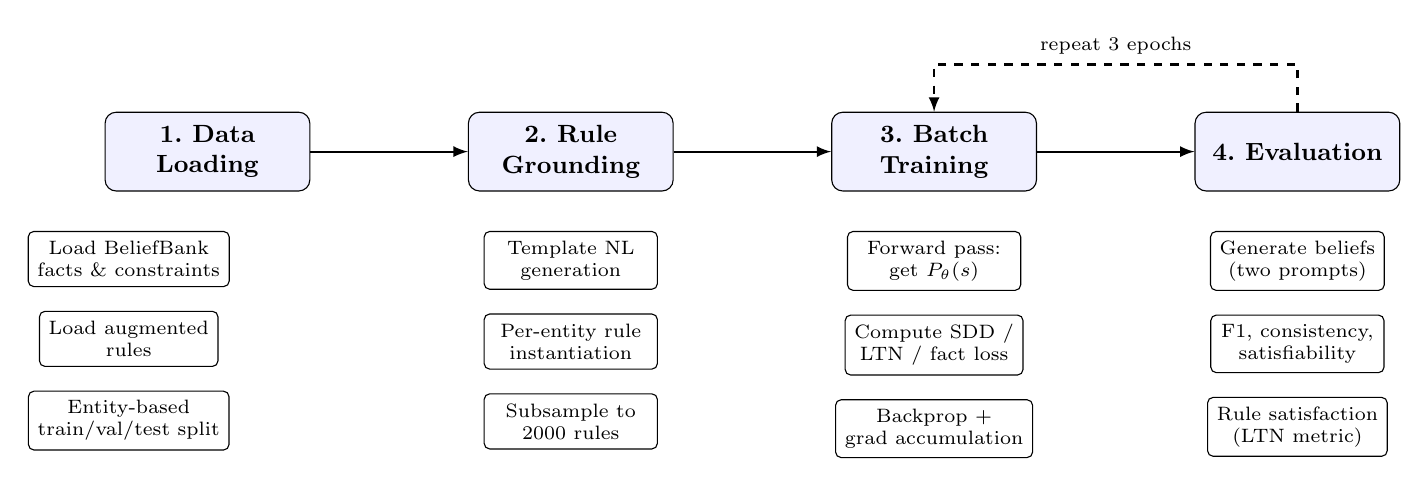
\begin{tikzpicture}[
    node distance=0.9cm,
    phase/.style={draw, rounded corners=4pt, minimum height=1.0cm,
                  minimum width=2.6cm, align=center, font=\small\bfseries,
                  fill=blue!6},
    substep/.style={draw, rounded corners=2pt, minimum height=0.7cm,
                    minimum width=2.2cm, align=center, font=\scriptsize},
    arr/.style={-latex, thick},
  ]
  % Phases
  \node[phase] (load) {1.\ Data\\Loading};
  \node[phase, right=2.0cm of load] (ground) {2.\ Rule\\Grounding};
  \node[phase, right=2.0cm of ground] (train) {3.\ Batch\\Training};
  \node[phase, right=2.0cm of train] (eval) {4.\ Evaluation};

  % Sub-steps
  \node[substep, below=0.5cm of load, xshift=-1.0cm] (s1a) {Load BeliefBank\\facts \& constraints};
  \node[substep, below=0.3cm of s1a] (s1b) {Load augmented\\rules};
  \node[substep, below=0.3cm of s1b] (s1c) {Entity-based\\train/val/test split};

  \node[substep, below=0.5cm of ground, xshift=-0.0cm] (s2a) {Template NL\\generation};
  \node[substep, below=0.3cm of s2a] (s2b) {Per-entity rule\\instantiation};
  \node[substep, below=0.3cm of s2b] (s2c) {Subsample to\\2000 rules};

  \node[substep, below=0.5cm of train, xshift=0.0cm] (s3a) {Forward pass:\\get $P_\theta(s)$};
  \node[substep, below=0.3cm of s3a] (s3b) {Compute SDD /\\LTN / fact loss};
  \node[substep, below=0.3cm of s3b] (s3c) {Backprop +\\grad accumulation};

  \node[substep, below=0.5cm of eval, xshift=0.0cm] (s4a) {Generate beliefs\\(two prompts)};
  \node[substep, below=0.3cm of s4a] (s4b) {F1, consistency,\\satisfiability};
  \node[substep, below=0.3cm of s4b] (s4c) {Rule satisfaction\\(LTN metric)};

  \draw[arr] (load) -- (ground);
  \draw[arr] (ground) -- (train);
  \draw[arr] (train) -- (eval);

  % dashed loop
  \draw[arr, dashed] (eval.north) -- ++(0,0.6) -| node[above,pos=0.25,font=\scriptsize]{repeat 3 epochs} (train.north);

\end{tikzpicture}%
}
\caption{Training pipeline.  Data is loaded and split by entity, rules are
  grounded into natural-language statements, batches pass through the
  combined loss, and evaluation runs after each epoch.}
\label{fig:pipeline}
\end{figure}

\subsection{Training Procedure}

All experiments fine-tune LLaMA~3.2-1B for 3~epochs on an NVIDIA~A100 GPU
through Google Colab.  \Cref{tab:hyperparams} lists the hyperparameters
for each configuration.

\begin{table}[H]
\centering
\caption{Hyperparameter settings for each training configuration.}
\label{tab:hyperparams}
\begin{tabular}{@{}lccc@{}}
\toprule
\textbf{Parameter} & \textbf{SDD} & \textbf{LTN} & \textbf{Hybrid} \\
\midrule
Learning rate          & $3{\times}10^{-4}$ & $1{\times}10^{-4}$ & $1{\times}10^{-4}$ \\
Batch size             & 128                & 16                  & 128                \\
Accumulation steps     & 1                  & 4                   & 1                  \\
Effective batch        & 128                & 4                   & 128                \\
$\lambda_{\text{sdd}}$ & 1.0 (implicit)     & N/A                 & 1.0                \\
$\lambda_{\text{ltn}}$ & N/A                & 5.0                 & 5.0                \\
$\lambda_{\text{fact}}$& N/A (implicit)     & 1.0                 & 1.0                \\
LoRA rank $r$          & 8                  & 8                   & 8                  \\
Implication floor $\gamma$ & N/A            & 0.5                 & 0.5                \\
pME power $p$          & N/A                & 2.0                 & 2.0                \\
Max training rules     & N/A                & 2000                & 2000               \\
Prob chunk size        & N/A                & 8                   & 8                  \\
Gradient clipping      & N/A                & 1.0                 & 1.0                \\
LR scheduler           & \multicolumn{3}{c}{CosineAnnealingLR}                       \\
Quantisation           & \multicolumn{3}{c}{4-bit NF4 (BitsAndBytes)}                \\
Epochs                 & \multicolumn{3}{c}{3}                                       \\
\bottomrule
\end{tabular}
\end{table}

\paragraph{SDD training loop.}
Each batch of grounded constraints is processed by: (1)~randomly selecting
one of two prompt formats, (2)~computing $P_\theta$ for antecedent,
consequent, and their negations, (3)~compiling the SDD formula per sample,
(4)~computing the semantic loss (\cref{eq:sdd}), and
(5)~backpropagating with gradient accumulation.

\paragraph{LTN training loop.}
For each batch of grounded rules: (1)~collect all unique statements
referenced in the batch, (2)~compute $P_\theta$ for each statement in
chunks of 8 (to fit GPU memory), (3)~evaluate each rule's fuzzy truth
value, (4)~aggregate via pMeanError and compute $\LTNloss$,
(5)~separately compute $\Lfact$ on a mini-batch of facts, and
(6)~backpropagate the weighted sum with gradient clipping at
$\|\nabla\|_{\max}{=}1.0$.

\paragraph{Hybrid training loop.}
This loop merges the two above.  SDD loss covers binary constraints, LTN
loss covers complex rules (\texttt{and\_implies}, \texttt{or\_implies},
\texttt{xor}), and a separate factual loss is computed on a fact
mini-batch.  The three terms are summed and backpropagated jointly.

\subsection{Evaluation Metrics}
\label{sec:metrics}

We evaluate along two axes: factual accuracy and logical
consistency.

\paragraph{Factual accuracy.}
\begin{itemize}[nosep]
  \item \textbf{F1 score}: the harmonic mean of precision and recall of the
    model's binary belief assignments against the ground-truth labels.
  \item \textbf{Antecedent / Consequent F1}: F1 computed separately on
    antecedent and consequent fact subsets, measuring whether the model
    preserves accuracy on both sides of constraints.
\end{itemize}

\paragraph{Logical consistency (SDD-based).}
Given a constraint $A \Rightarrow B$:
\begin{itemize}[nosep]
  \item \textbf{Consistency}: when the reference believes~$A$, does the
    model's belief about~$B$ match the constraint's expected value?
  \item \textbf{Inverse consistency}: when the model believes $\lnot B$,
    does it also believe $\lnot A$?  (Contrapositive check.)
  \item \textbf{Multi-hop consistency}: for 2-hop chains
    $A \Rightarrow B \Rightarrow C$, when both $A$ and $B$ are believed,
    does the model's belief about~$C$ match?
  \item \textbf{Satisfiability}: does the model's joint assignment
    $(A, B)$ lie in the truth table of the implication formula?
  \item \textbf{Negation consistency}: does $P(s) \neq P(\lnot s)$
    for every statement~$s$ and its negation?
\end{itemize}

\paragraph{Rule satisfaction (LTN-based).}
Average rule satisfaction is the mean fuzzy truth value across all
applicable grounded rules, using the model's binary beliefs as crisp
inputs.  It tells us how well the model respects the full augmented rule
set, including complex rules that the SDD metrics cannot capture.

% ======================================================================
% 3  EXPERIMENTAL RESULTS
% ======================================================================
\section{Experimental Results}

\subsection{Experimental Setup}

All four configurations share the same LLaMA~3.2-1B backbone, the same
BeliefBank data splits, and the same entity-based subsampling (30~entities
for evaluation).  We evaluate with two prompt formats on two fact sets
(calibration and silver).  The main tables report the average across both
prompts; per-prompt breakdowns are included for completeness.

\subsection{Performance of Different Approaches}

\Cref{tab:main-cal,tab:main-silver} present the full results on
calibration and silver facts respectively.

% ====== calibration results ======
\begin{table}[H]
\centering
\caption{Test results on \textbf{calibration} facts (average of prompt~0
  and prompt~1).  Best value in each column is \textbf{bolded}.
  ``N/A'' indicates the metric is not available for that configuration.}
\label{tab:main-cal}
\small
\begin{tabular}{@{}lcccc@{}}
\toprule
\textbf{Metric} & \textbf{Base} & \textbf{LTN} & \textbf{SDD} & \textbf{Hybrid} \\
\midrule
F1                          & 0.17  & 0.28  & \textbf{0.88} & 0.74 \\
Negation consistency        & 0.21  & 0.32  & \textbf{0.95} & 0.85 \\
Avg.\ rule satisfaction     & 0.65  & 0.62  & 0.59          & \textbf{0.70} \\
\midrule
Self-consistency            & N/A   & N/A   & \textbf{0.87} & 0.77 \\
Self-inverse consistency    & N/A   & N/A   & \textbf{0.94} & 0.90 \\
Self-multihop consistency   & N/A   & N/A   & \textbf{0.94} & 0.84 \\
Consistency (ref)           & N/A   & N/A   & \textbf{0.87} & 0.77 \\
Inverse consistency (ref)   & N/A   & N/A   & \textbf{0.94} & 0.90 \\
Multihop consistency (ref)  & N/A   & N/A   & \textbf{0.94} & 0.84 \\
Satisfiability              & N/A   & N/A   & \textbf{0.98} & 0.96 \\
\midrule
Antecedents F1              & 0.09  & 0.07  & \textbf{0.91} & 0.78 \\
Consequents F1              & 0.21  & 0.44  & \textbf{0.84} & 0.74 \\
\bottomrule
\end{tabular}
\end{table}

% ====== silver results ======
\begin{table}[H]
\centering
\caption{Test results on \textbf{silver} facts (average of prompt~0
  and prompt~1).  Best value in each column is \textbf{bolded}.}
\label{tab:main-silver}
\small
\begin{tabular}{@{}lcccc@{}}
\toprule
\textbf{Metric} & \textbf{Base} & \textbf{LTN} & \textbf{SDD} & \textbf{Hybrid} \\
\midrule
F1                          & 0.17  & 0.26  & \textbf{0.77} & 0.62 \\
Negation consistency        & 0.19  & 0.31  & \textbf{0.95} & 0.90 \\
Avg.\ rule satisfaction     & \textbf{0.69}  & 0.68  & 0.55 & 0.69 \\
\midrule
Self-consistency            & N/A   & N/A   & \textbf{0.83} & 0.73 \\
Self-inverse consistency    & N/A   & N/A   & \textbf{0.93} & 0.89 \\
Self-multihop consistency   & N/A   & N/A   & \textbf{0.92} & 0.79 \\
Consistency (ref)           & N/A   & N/A   & \textbf{0.76} & 0.67 \\
Inverse consistency (ref)   & N/A   & N/A   & \textbf{0.93} & 0.89 \\
Multihop consistency (ref)  & N/A   & N/A   & \textbf{0.92} & 0.83 \\
Satisfiability              & N/A   & N/A   & \textbf{0.98} & 0.96 \\
\midrule
Antecedents F1              & 0.07  & 0.08  & \textbf{0.85} & 0.68 \\
Consequents F1              & 0.23  & 0.43  & \textbf{0.72} & 0.60 \\
\bottomrule
\end{tabular}
\end{table}

% ====== per-prompt detail table ======
\begin{table}[H]
\centering
\caption{Per-prompt breakdown of key metrics on calibration facts.
  Prompt~0 uses ``true''/``false'' labels; Prompt~1 uses ``yes''/``no''.}
\label{tab:per-prompt}
\small
\begin{tabular}{@{}ll cccc@{}}
\toprule
\textbf{Prompt} & \textbf{Metric} & \textbf{Base} & \textbf{LTN} & \textbf{SDD} & \textbf{Hybrid} \\
\midrule
\multirow{3}{*}{0}
  & F1              & 0.18 & 0.14 & 0.88 & 0.71 \\
  & Neg.\ consist.  & 0.23 & 0.14 & 0.94 & 0.86 \\
  & Rule sat.       & 0.62 & 0.63 & 0.58 & 0.69 \\
\midrule
\multirow{3}{*}{1}
  & F1              & 0.16 & 0.43 & 0.89 & 0.77 \\
  & Neg.\ consist.  & 0.18 & 0.50 & 0.96 & 0.85 \\
  & Rule sat.       & 0.68 & 0.62 & 0.60 & 0.72 \\
\bottomrule
\end{tabular}
\end{table}

% ======================================================================
%  BAR CHARTS
% ======================================================================

\begin{figure}[H]
\centering
\subfloat[Factual accuracy (F1).\label{fig:f1-bar}]{%
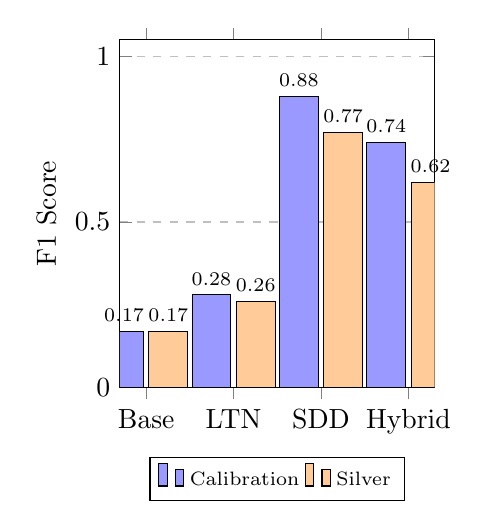
\begin{tikzpicture}
\begin{axis}[
    ybar, bar width=14pt,
    width=0.46\textwidth, height=6cm,
    ylabel={F1 Score},
    symbolic x coords={Base,LTN,SDD,Hybrid}, xtick=data,
    ymin=0, ymax=1.05,
    ymajorgrids=true, grid style={dashed},
    nodes near coords, nodes near coords style={font=\scriptsize,above},
    every node near coord/.append style={/pgf/number format/.cd,fixed,precision=2},
    legend style={at={(0.5,-0.20)},anchor=north,legend columns=2,font=\scriptsize},
]
\addplot[fill=blue!40] coordinates {(Base,0.17)(LTN,0.28)(SDD,0.88)(Hybrid,0.74)};
\addplot[fill=orange!40] coordinates {(Base,0.17)(LTN,0.26)(SDD,0.77)(Hybrid,0.62)};
\legend{Calibration,Silver}
\end{axis}
\end{tikzpicture}%
}\hfill
\subfloat[Negation consistency.\label{fig:neg-bar}]{%
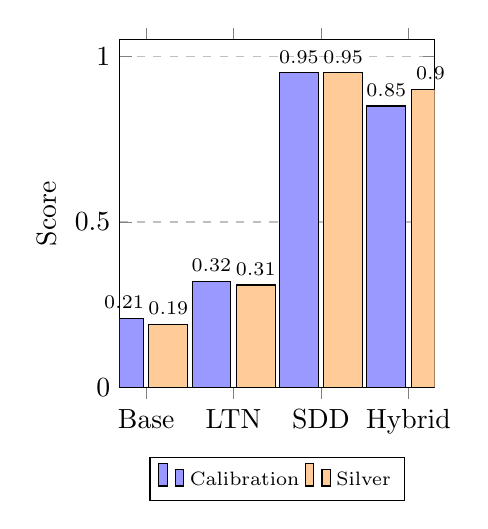
\begin{tikzpicture}
\begin{axis}[
    ybar, bar width=14pt,
    width=0.46\textwidth, height=6cm,
    ylabel={Score},
    symbolic x coords={Base,LTN,SDD,Hybrid}, xtick=data,
    ymin=0, ymax=1.05,
    ymajorgrids=true, grid style={dashed},
    nodes near coords, nodes near coords style={font=\scriptsize,above},
    every node near coord/.append style={/pgf/number format/.cd,fixed,precision=2},
    legend style={at={(0.5,-0.20)},anchor=north,legend columns=2,font=\scriptsize},
]
\addplot[fill=blue!40] coordinates {(Base,0.21)(LTN,0.32)(SDD,0.95)(Hybrid,0.85)};
\addplot[fill=orange!40] coordinates {(Base,0.19)(LTN,0.31)(SDD,0.95)(Hybrid,0.90)};
\legend{Calibration,Silver}
\end{axis}
\end{tikzpicture}%
}

\vspace{1em}

\subfloat[SDD-based consistency metrics (calibration).\label{fig:consist-bar}]{%
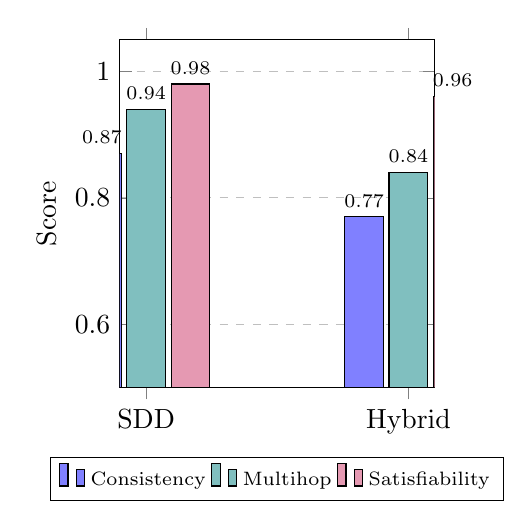
\begin{tikzpicture}
\begin{axis}[
    ybar, bar width=14pt,
    width=0.46\textwidth, height=6cm,
    ylabel={Score},
    symbolic x coords={SDD,Hybrid}, xtick=data,
    ymin=0.5, ymax=1.05,
    ymajorgrids=true, grid style={dashed},
    nodes near coords, nodes near coords style={font=\scriptsize,above},
    every node near coord/.append style={/pgf/number format/.cd,fixed,precision=2},
    legend style={at={(0.5,-0.20)},anchor=north,legend columns=3,font=\scriptsize},
]
\addplot[fill=blue!50] coordinates {(SDD,0.87)(Hybrid,0.77)};
\addplot[fill=teal!50] coordinates {(SDD,0.94)(Hybrid,0.84)};
\addplot[fill=purple!40] coordinates {(SDD,0.98)(Hybrid,0.96)};
\legend{Consistency,Multihop,Satisfiability}
\end{axis}
\end{tikzpicture}%
}\hfill
\subfloat[Average rule satisfaction (LTN metric).\label{fig:rule-bar}]{%
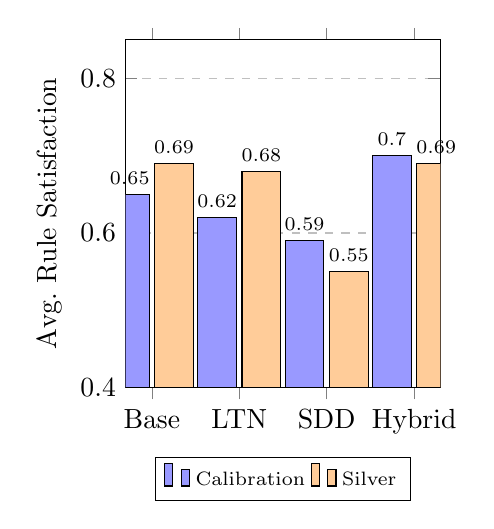
\begin{tikzpicture}
\begin{axis}[
    ybar, bar width=14pt,
    width=0.46\textwidth, height=6cm,
    ylabel={Avg.\ Rule Satisfaction},
    symbolic x coords={Base,LTN,SDD,Hybrid}, xtick=data,
    ymin=0.4, ymax=0.85,
    ymajorgrids=true, grid style={dashed},
    nodes near coords, nodes near coords style={font=\scriptsize,above},
    every node near coord/.append style={/pgf/number format/.cd,fixed,precision=2},
    legend style={at={(0.5,-0.20)},anchor=north,legend columns=2,font=\scriptsize},
]
\addplot[fill=blue!40] coordinates {(Base,0.65)(LTN,0.62)(SDD,0.59)(Hybrid,0.70)};
\addplot[fill=orange!40] coordinates {(Base,0.69)(LTN,0.68)(SDD,0.55)(Hybrid,0.69)};
\legend{Calibration,Silver}
\end{axis}
\end{tikzpicture}%
}
\caption{Comparison of all four model configurations across key metrics.}
\label{fig:all-bars}
\end{figure}

% ======================================================================
% 4  ANALYSIS AND DISCUSSION
% ======================================================================
\section{Analysis and Discussion}

\subsection{SDD Dominance on Factuality and Consistency}

The SDD-only model leads on every factuality and consistency metric.  Its
semantic loss (\cref{eq:sdd}) works in an exact probabilistic regime. It enumerates all satisfying worlds, so the gradient signal is
precise.  The loss also conditions on ground-truth labels when they are
available, which effectively folds factual supervision and logical
regularisation into one term.  A large batch size (128) keeps gradient
estimates stable, and the higher learning rate ($3{\times}10^{-4}$) lets
the model converge within the 3-epoch budget.

\subsection{LTN Convergence Failure}

The LTN-only model performs worst among the trained configurations.  Its
F1 actually drops below the untrained base on prompt~0
(0.14 vs.\ 0.18).  We trace this to three interacting causes:

\paragraph{Logic weight sensitivity.}
At $\lambda_{\text{ltn}}{=}5$ and $\lambda_{\text{fact}}{=}1$ the fuzzy
logic loss dominates the objective.  The model learns to output
near-constant probabilities (all low or all high) that satisfy many rules
vacuously.  Predicting $P_\theta(s){\approx}0$ for every statement, for
example, makes most implications trivially true because the antecedent is
false, but it destroys factual accuracy.

Setting the logic weight lower (e.g.\ $\lambda_{\text{ltn}}{=}1$)
produces the opposite problem. Not enough constraint pressure, and the
model converges to a purely factual solution with no logical gain.
Finding the right balance proved difficult within our hyperparameter
budget.

\paragraph{Small effective batch size.}
Memory constraints forced an effective batch size of 4 (batch~16 with
4$\times$ gradient accumulation), producing high-variance gradients.
The SDD and hybrid configurations use batch~128, yielding far more stable
updates.

\paragraph{Probability chunking overhead.}
Computing $P_\theta$ for every unique statement in a rule batch requires
processing them in chunks of~8 due to memory limits.  This issues many
small forward passes, which slows training.  Worse, each backward pass
only sees a fraction of the constraint graph, so the gradient signal
lacks coherence.

\subsection{Hybrid Trade-offs}

The hybrid model reaches the \textbf{highest average rule satisfaction}
(0.70 on calibration, 0.69 on silver).  This confirms that the LTN
component adds meaningful gradient signal for complex rules SDDs cannot
handle.  On the other hand, factuality (F1\,=\,0.74 on calibration) and
consistency fall short of SDD-only.  We attribute this to loss
interference. Three loss terms ($\SL$, $\LTNloss$, $\Lfact$) compete
for the limited capacity of the LoRA adapters ($r{=}8$).  The LTN loss
sometimes pushes probabilities in directions that conflict with the SDD
signal.

\subsection{Design Challenges}

\paragraph{SDD edge cases.}
The SDD loss compiles one formula per sample and enumerates its models.
If a formula becomes unsatisfiable after conditioning on ground-truth
labels, there are no satisfying worlds and the sum in \cref{eq:sdd} hits
zero.  We fall back to $-\log(\epsilon)$, but these samples still
produce uninformative constant gradients.  Before we added this fallback,
the result was \texttt{NaN} losses during training.

\paragraph{Batch construction asymmetry.}
SDD constraints are grounded per-entity and loaded through a standard
\texttt{DataLoader}, giving uniform batches of~128.  LTN rules are
different: a single \texttt{universal} rule touches 2~statements, while a
complex \texttt{and\_implies} may touch 4 or more.  This makes GPU memory
usage unpredictable from batch to batch.  Our workaround is
\texttt{prob\_chunk\_size\,=\,8}, which processes 8~statements at a time
but adds sequential overhead.

\paragraph{Prompt sensitivity.}
\Cref{tab:per-prompt} shows that the choice of prompt format
(``true''/``false'' vs.\ ``yes''/``no'') matters a lot.  The LTN model's
F1 jumps from 0.14 to 0.43 just by switching from prompt~0 to prompt~1.
This suggests the model's token biases interact unpredictably with the
logic loss and points to the need for prompt-robust training or an
instruction-tuned base model.

% ======================================================================
% 5  LIMITATIONS AND FUTURE WORK
% ======================================================================
\section{Limitations and Future Work}

\paragraph{Instruct-tuned base models.}
We use the raw LLaMA~3.2-1B base model, which has poor zero-shot
instruction following.  An instruct-tuned variant (e.g.\
Llama-3.2-1B-Instruct) would give a stronger starting point for
factuality and lower prompt sensitivity.

\paragraph{Prompt diversity.}
We train and evaluate on only two prompt formats.  Testing with a wider
range of templates, including few-shot prompts, would reveal how robust
the approach is to surface-form variation.

\paragraph{LTN hyperparameter tuning.}
The LTN-only configuration suffers from a coarse hyperparameter search.
A curriculum-style schedule for $\lambda_{\text{ltn}}$, starting low and
ramping up over epochs, could let the model learn factual accuracy first
before logic regularisation kicks in.

\paragraph{Log-space fuzzy operators.}
The logLTN framework~\cite{logltn2023} runs fuzzy operators in logarithm
space to avoid the vanishing products and underflow that plague the
standard product t-norm when many conjuncts are involved.  Adopting
logLTN could improve LTN training stability.

\paragraph{Larger models and datasets.}
Scaling to larger LLMs (7B+) and richer knowledge bases would show
whether these patterns hold more broadly.  Larger LoRA ranks and longer
training may also help the hybrid model overcome loss interference.

\paragraph{Inference-time reasoning.}
Our approach bakes logical constraints into the training loss.  At
inference time the model relies only on its learned parameters.  A
natural extension would pair training-time LTN regularisation with
lightweight inference-time constraint propagation.

% ======================================================================
% 6  CONCLUSION
% ======================================================================
\section{Conclusion}

We set out to test whether Logic Tensor Networks can make LLM outputs
more logically consistent.  The idea is to add differentiable fuzzy-logic
constraints to the fine-tuning objective.  We ran experiments on
BeliefBank with LLaMA~3.2-1B across four configurations: an untrained
base model, an SDD model with propositional semantic loss, an LTN-only
model with fuzzy first-order logic loss, and a hybrid that combines both.

SDD proved most effective overall.  It reached an F1 of 0.88 and
consistency of 0.87 on calibration facts, roughly $5\times$ better than
the untrained baseline.  The hybrid model showed that LTN constraints add
real value for complex rules (highest rule satisfaction at 0.70), but at
the cost of lower factuality compared to SDD alone.  LTN-only failed to
converge, largely because of sensitivity to the logic-weight
hyperparameter and the small batch sizes forced by memory limits.

The takeaway is that exact probabilistic constraints (SDDs) still
beat approximate fuzzy methods (LTNs) when the rules fit in
propositional logic.  For richer first-order rules that SDDs cannot
handle efficiently, the hybrid approach is a workable alternative.
Future work should explore curriculum-based weight scheduling,
instruct-tuned base models, and log-space fuzzy operators to narrow
the gap between LTN and SDD performance.

% ======================================================================
% 7  CONTRIBUTIONS
% ======================================================================
\section{Author Contributions}

This project was a joint effort between Travis Tran and Anishwar
Chakraborty.  We began by jointly studying the LoCo-LM
codebase~\cite{calanzone2025loco} and deciding which pieces to reuse and
which to build from scratch.

\paragraph{Travis Tran.}
Travis led the data-augmentation pipeline: he prompted an LLM with
per-entity truth tables to generate the augmented rule set (XOR,
AND-implies, OR-implies, equivalence, universal) and validated the
generated rules against silver-fact labels.  He also implemented and
debugged the SDD training loop, including the constraint manager, the
four SDD modes (implication, inverse implication, negation, all), and
the edge-case handling for unsatisfiable formulas that initially caused
\texttt{NaN} losses.

\paragraph{Anishwar Chakraborty.}
Anishwar designed and implemented the LTN training pipeline: the fuzzy
connectives (product t-norm, probabilistic sum, floored Reichenbach
implication, equivalence), the pMeanError aggregation, the rule-grounding
logic, and the probability-chunking workaround for GPU memory.  He also
built the hybrid training loop that merges SDD and LTN losses and ran
the evaluation across all four configurations.

% ======================================================================
% REFERENCES
% ======================================================================
\bibliographystyle{plainnat}

\begin{thebibliography}{10}

\bibitem{calanzone2025loco}
Diego Calanzone, Stefano Teso, and Antonio Vergari.
\newblock Logically consistent language models via neuro-symbolic integration.
\newblock In \emph{Proceedings of the International Conference on Learning
  Representations (ICLR)}, 2025.

\bibitem{badreddine2022ltn}
Samy Badreddine, Artur~d'Avila Garcez, Luciano Serafini, and Michael Spranger.
\newblock Logic {T}ensor {N}etworks.
\newblock \emph{Artificial Intelligence}, 303:103649, 2022.

\bibitem{ltntorch2024}
Tommaso Carraro, Benedikt Wagner, Samy Badreddine, and Alessandro Daniele.
\newblock {LTNtorch}: {P}y{T}orch implementation of {L}ogic {T}ensor
  {N}etworks.
\newblock \emph{arXiv preprint arXiv:2409.16045}, 2024.

\bibitem{kassner2021beliefbank}
Nora Kassner, Oyvind Tafjord, Hinrich Sch\"{u}tze, and Peter Clark.
\newblock {BeliefBank}: Adding memory to a pre-trained language model for a
  systematic notion of belief.
\newblock In \emph{Proceedings of the Conference on Empirical Methods in
  Natural Language Processing (EMNLP)}, pages 8707--8718, 2021.

\bibitem{xu2018semantic}
Jingyi Xu, Zilu Zhang, Tal Friedman, Yitao Liang, and Guy Van~den Broeck.
\newblock A semantic loss function for deep learning with symbolic knowledge.
\newblock In \emph{Proceedings of the International Conference on Machine
  Learning (ICML)}, pages 5502--5511, 2018.

\bibitem{darwiche2011sdd}
Adnan Darwiche.
\newblock {SDD}: A new canonical representation of propositional knowledge
  bases.
\newblock In \emph{Proceedings of the International Joint Conference on
  Artificial Intelligence (IJCAI)}, pages 819--826, 2011.

\bibitem{logltn2023}
Alessandro Daniele, Tommaso Campari, Samy Badreddine, and Luciano Serafini.
\newblock {logLTN}: Differentiable fuzzy logic in the logarithm space.
\newblock \emph{arXiv preprint arXiv:2306.14546}, 2023.

\bibitem{llama32}
Meta AI.
\newblock {L}lama 3.2: Lightweight text and multimodal models.
\newblock \url{https://ai.meta.com/blog/llama-3-2-connect-2024-vision-edge-mobile-devices/}, 2024.

\bibitem{hu2022lora}
Edward~J. Hu, Yelong Shen, Phillip Wallis, Zeyuan Allen-Zhu, Yuanzhi Li,
  Shean Wang, Lu~Wang, and Weizhu Chen.
\newblock {LoRA}: Low-rank adaptation of large language models.
\newblock In \emph{Proceedings of the International Conference on Learning
  Representations (ICLR)}, 2022.

\bibitem{dettmers2023qlora}
Tim Dettmers, Artidoro Pagnoni, Ari Holtzman, and Luke Zettlemoyer.
\newblock {QLoRA}: Efficient finetuning of quantized language models.
\newblock In \emph{Advances in Neural Information Processing Systems
  (NeurIPS)}, 2023.

\end{thebibliography}

% ======================================================================
% APPENDIX
% ======================================================================
\appendix
\section{Code Repository}

The full source code for this project, including training scripts,
configuration files, evaluation utilities, and the augmented rule set,
is publicly available at:

\begin{center}
\url{https://github.com/travis-tran03/CS273P-LTN-LLM}
\end{center}

\end{document}
